\documentclass[11pt]{article}
\usepackage{geometry}                
\geometry{letterpaper}                   

\usepackage{listings}
\usepackage{color}
\usepackage{graphicx}
\usepackage{epstopdf}
\usepackage{varioref}
\usepackage[numbers]{natbib}
\usepackage[squaren]{SIunits}
\usepackage{amssymb, amsmath}

\DeclareGraphicsRule{.tif}{png}{.png}{`convert #1 `dirname #1`/`basename #1 .tif`.png}

\title{Modelling Situations of Evacuation in a Multi-level Building}
\author{Hans Hardmeier, Andrin Jenal, Beat K\"ung & Felix Thaler}
\date{date} 

\begin{document}



\thispagestyle{empty}

\begin{center}

\includegraphics[width=5cm]{ETHlogo.eps}

\bigskip


\bigskip


\bigskip


\LARGE{ 	Lecture with Computer Exercises:\\ }
\LARGE{ Modelling and Simulating Social Systems with MATLAB\\}

\bigskip

\bigskip

\small{Project Report}\\

\bigskip

\bigskip

\bigskip

\bigskip


\begin{tabular}{|c|}
\hline
\\
\textbf{\LARGE{Insert Title Here}}\\
\textbf{\LARGE{...}}\\
\\
\hline
\end{tabular}
\bigskip

\bigskip

\bigskip

\LARGE{Name 1 \& Name 2}



\bigskip

\bigskip

\bigskip

\bigskip

\bigskip

\bigskip

\bigskip

\bigskip

Zurich\\
March 2012\\

\end{center}



\newpage

%%%%%%%%%%%%%%%%%%%%%%%%%%%%%%%%%%%%%%%%%%%%%%%%%

\newpage
\section*{Agreement for free-download}
\bigskip


\bigskip


\large We hereby agree to make our source code for this project freely available for download from the web pages of the SOMS chair. Furthermore, we assure that all source code is written by ourselves and is not violating any copyright restrictions.

\begin{center}

\bigskip
\bigskip
\bigskip
\bigskip


\begin{tabular}{@{}p{3.3cm}@{}p{6cm}@{}@{}p{6cm}@{}}

\begin{minipage}{3cm}

\end{minipage}
&
\begin{minipage}{6cm}
\vspace{2mm} \large Hans Hardmeier

 \vspace{\baselineskip}

\end{minipage}
&
\begin{minipage}{6cm}

\large Andrin Jenal

\end{minipage}

\end{tabular}

\bigskip
\bigskip
\bigskip
\bigskip


\begin{tabular}{@{}p{3.3cm}@{}p{6cm}@{}@{}p{6cm}@{}}

\begin{minipage}{3cm}

\end{minipage}
&
\begin{minipage}{6cm}
\vspace{2mm} \large Beat K\"ung

 \vspace{\baselineskip}

\end{minipage}
&
\begin{minipage}{6cm}

\large Felix Thaler

\end{minipage}
\end{tabular}

\end{center}
\newpage

%%%%%%%%%%%%%%%%%%%%%%%%%%%%%%%%%%%%%%%



% IMPORTANT
% you MUST include the ETH declaration of originality here; it is available for download on the course website or at http://www.ethz.ch/faculty/exams/plagiarism/index_EN; it can be printed as pdf and should be filled out in handwriting

%TODO: The is declaration of originality on the WEb for Windows (Andrin Jenal)...

%%%%%%%%%% Table of content %%%%%%%%%%%%%%%%%

\tableofcontents

\newpage

%%%%%%%%%%%%%%%%%%%%%%%%%%%%%%%%%%%%%%%



\section{Abstract}

If you are an ETH-Student, you know that at lunch time it is almost impossible 
to go out of the building through the main entrance to the polyterasse, because
of the number of students trying to leave at the same time. What would happen,
if in addition to that, an evacuation was involved? Have you ever imagined, how
an evacuation at the ETH Main building, ETH CAB-Building or even at your own home
would look like? How many people would be able to leave simultaneously? What is the
best strategy for people to leave? How would the perfect evacuation plan for your
school or enterprise building look like?

In this work, we decided to elaborate a program that is flexible enough to
calculate the fastest exit for every given building structure. Using a "2D Range Tree Datastructure" 
to improve the access to the forces over each agent and solve this complex problem, the program is capable of computing the fastest way
very efficiently.


Different from all other similar projects, we also focused on an efficient and
realistic implementation of the program. For the preprocessing, the "Fast Sweeping Algorithm Method" 
enable us to have only some seconds of initialization time (instead of some minutes with "Fast Marching Algorithm". 
See \ref{implementation}) and using our own "2D Range Tree" data structures, to
handle the numerous amount of agents, enables us to simulate large buildings with many agents and
with a realistic force model.

\section{Individual contributions}

We all worked together in this project and used the individual strengths of each
of us to achieve the best possible result. Detailed information about the
contribution of each of us can be obtained from the git history.

Carl Hans Peter Hardmeier Samame, alias Hans Hardmeier, was 
responsible for some parts of the documentation, verification of the MATLAB-code
and calculating efficienty using different operating systems (i.e. Mac OS 10.6).

Contributing to some core functionalities of the social force model, especially repulsive effects, Andrin Jenal focused on the moddeling of the buildings layout used in the simulation. Additionally, he elaborated some sections of the documentation.

Beat K\"ung did most of the plotting functionality and the definition \&
implementation of the configuration and building image file. He also did several
sections of the documentation.

Felix Thaler implemented the algorithms written in \textit{C}, using \textit{MATLAB}'s \textit{MEX}-interface.
These are efficient \textit{Fast Sweeping}, a 2D \textit{Range Tree} and fast bilinear interpolation.
Further he developed the basic simulation framework and added the social force model as well as some
custom algorithms, for instance one to minimize wall penetration of agents. Some sections of the documentation are
written by him, too.


\section{Introduction and Motivations}

\subsection{Introduction}

Simulating the evacuation scenario of a single-level building is well known but
is not general enough. Though we want to introduce a more sophisticated
simulation within a multi-level building. E.g.: What would happen, if a
multi-level building has to be evacuated? Which escape routes would be mostly
used? Which effects would have the pressure of other persons to the
situation? Since tower buildings are getting more common in large cities,
engineers have to care more about the behaviour in situations of emergency,
namely evacuations. Apart of the mathematical model and implementation for
solving this problem, we also wanted to increase the utility of this program for
all readers by giving the possibility of calculate different scenarios in
different buildings given by the user. In this work, we will mostly work with
the map of the ETH building, however, there are more configurations in the data
folder and one can replace any map with others that meet the properties of the
Figure \ref{building floor image} in the section \ref{matlab code}.

\subsection{Motivation}

Intuitive expectations and mathematical model results can stay sometimes in
contradiction. Our intuition is full of little contepts that are hard to realize in a concient way.
Using the language of mathematics, we want to describe formaly all the elements that contribute
to the complex result of the human behavior. However, a common point of motivation within the group is 
the connection between the 'real' World and the mathematical formalism.

On ther other side, we, as ETH-Students, are not sure, if the evacuation
potential (the property of a buiding of being evacuated efficiently) of our ETH-buildings are enough for the amount of students during a normal
week day and on the other hand, we want to help the people around the world,
that have a similar question, to find an answer. This two points gave us the
ideas and motivation to create a flexible tool that simulates a real-world
scenario for any given building or even structures (i.e. planes or boats).


\subsection{Fundamental Questions}

In the first place, we all are wondering \textit{how exaclty an implementation of a social force model looks like}, based on already published papers coping with this problem \cite{SFMPD} \cite{SDFEP}. Of special interest is also \textit{how this model can be implemented efficiently for a multilevel building and how it can be extended to add some dynamic features}. Moreover are we keen to understand \textit{how the simulation behaves applying the model to a real building like the ETH main building}. Generally speaking, \textit{how realistic is the behaviour of the agents used in our model?}.

\section{Description of the Model}
\subsection{General Model}

For our model, we will create a relatively general framework for behavioral
simulation in evacuation scenarios based on the social force model introduced by Dirk Helbling \cite{SDFEP}.
A core investigation is a simulation, beginning in a general everyday situation,
where people are spread randomly in their office or somewhere in the hallway and ending in an evacuation scenario.
At the end we should be able to make strong
statements anwsering our fundamental questions.
Based on the forces explained in the following paragraphs, we tried to figure
out how agents overcome major obstacles like tiny passages, stairs or pillars. Whereas, the
shape and complexity of rooms and building is a key factor, contributing to the behaviour of the
agents as well. % Do we need this last sentence?

\subsection {Forces}
The reactions of the agents will mainly be influenced by different forces, model
parameters and the building structure itself. 
Describing this problem in mathematical terms, leads to an equation, where the mass, the desired direction $f_{D}$, the repulsive forces $f_{ij}$ and the wall force $f_{iW}$ of each individual agent contribute to the change of velocity in time.\\
Helbling stated this problem as the following:"We assume a mixture of socio-psychological and physical forces influencing the behaviour in a crowd: each of $N$ pedestrians $i$ of mass $m_{i}$ likes to move with a certain desired speed $v_{i}^0$ in a certain direction $\mathbf{e}_{i}^0$, and therefore tends to correspondingly adapt his or her actual velocity $\mathbf{v}_i$ with a certain characteristic time $\tau_{i}$. Simulataneously, he or she tries to keep a velocity-dependent distance from other pedestrians $j$ and walls $W$."

\begin{equation} \label{eq:eikonal}
m_{i}\frac{\mathsf{d}\mathbf{v}_{i}}{\mathsf{d}t}=m_{i}f_{D}+\sum \limits_{j(\neq{i})}{f_{ij}}+\sum \limits_{W}{f_{iW}}, f_{D}=\frac{v_{i}^{0}(t)\mathbf{e}_{i}^{0}(t)-\mathbf{v}_{i}(t)}{\tau_{i}}
\end{equation}

That means the change of position $\mathbf{r}$ is given by the velocity: $\mathbf{v}_{i}=\frac{\mathsf{d}\mathbf{r}_{i}}{\mathsf{d}t}$\\
To understand the different party, they will be explained briefly.

% [comment (Felix): we need to write MUCH more cleary that all these forces are exactly the same as the one proposed by Helbling!! This is my no means our work!]

\subsubsection{Desired Direction}

% [comment (Felix): ääääh somewhat short?? :-P]
%todo: merge with path finding (felix)
\begin{equation} \label{eq:eikonal}
F_{D}=m\frac{v(t)\mathbf{e(t)}-\mathbf{v(t)}}{\tau}
\end{equation}

\subsubsection{Repulsive Interaction Force}

As people don't like to get too close to each other, the main component of this
formula is a rather psychological aspect and plays an important role to keep
agents apart from each other. However if it should happen that agents get too
close, two additional forces, the 'body force' counteracting body compression
and 'sliding friction force' contribute to the repulsive force to ensure a
certain distance. \cite{SDFEP} 

\begin{equation} \label{eq:eikonal}
f_{ij}=\left\{A_{i}exp[(r_{ij}-d_{ij})/B_{i}]+kg(r_{ij}-d_{ij})\right\}\mathbf{n}_{ij}+\kappa g(r_{ij}-d_{ij})\triangle v_{ji}^t\mathbf{t}_{ij}
\end{equation}

According to Helbling the repulsive interaction force $A_{i}exp[(r_{ij}-d_{ij})/B_{i}]\mathbf{n}_{ij}$ describes the psychological tendency of two pedestrians $i$ and $j$ to stay away from each other, where $A_i$ and $B_i$ are constants. 
"$d_{ij}=\|r_i-r_j\|$ denotes the distance between the pedestrians' centres of mass, and $\mathbf{n}_{ij}=(n_{ij}^1, n_{ij}^2)=\mathbf{r_i}-\mathbf{r_j}/d_{ij}$ is the normalized vector pointing from pedestrian $j$ to $i$.
The pedestrians touch each other if their distance $d_{ij}$ is smaller than the sum $r_{ij}=(r_i+r_j)$ of their radii $r_i$ and $r_j$."\cite{SDFEP}
If this is the case two addtional forces are considered:
$k(r_{ij}-d_{ij})\mathbf{n}_{ij}$ and $\kappa(r_{ij}-d_{ij})\triangle
v_{ij}^t\mathbf{t}_{ij}$. "Here $\mathbf{t}_{ij}=(-n_{ij}^2,n_{ij}^1)$ means
the tangential direction and $\triangle
v_{ij}^t=(\mathbf{v}_j-\mathbf{v}_i)\cdot\mathbf{t}_{ij}$ and the function
$g(x)$ is zero if the pedestrians do not touch each other $(d_{ij}>r_{ij})$,
and otherwise equal to the argument $x$."\cite{SDFEP}

\subsubsection{Wall Force}

To prevent agents walking into or even through walls, there exists a wall force normal to the wall such that the closer agents gets to walls the stronger gets the tangential force.
Helbling states it the following:"$d_{iW}$ means the distance to wall $W$, $\mathbf{n}_{iW}$ denotes  the direction perpendicular to it, and $\mathbf{n}_{iW}$ the direction tangential to it, the corresponding interaction force with the wall is given by:" \cite{SFMPD}

\begin{equation} \label{eq:eikonal}
f_{iW}=\left\{A_{i}exp[(r_{i}-d_{iW})/B_{i}]+kg(r_{i}-d_{iW})\right\}\mathbf{n}_{iW}-\kappa g(r_{i}-d_{iW})(\mathbf{v}_{i}\cdot\mathbf{t}_{iW})\mathbf{t}_{iW}
\end{equation}

\section{Implementation}\label{implementation}
Our goal was a fast implementation of the model. So we decided to use the Fast
Sweeping algorithm instead of the Fast Marching alorithm to calculate the
fastest way out of a building. We knew that \textit{MATLAB} code is not very fast and
\textit{MATLAB} provides an interface for other programming languages. So we
used the \textit{C} programming language to implement the Fast Sweeping method.

Later in the development process we discovered another bottleneck in our code:
The social force between the agents which runs in $ O(N^2) $. Felix Thaler then
introduced a Range Tree for this problem, which he also implemented in
\textit{C}.


\subsection{\textit{MATLAB} Code} \label{matlab code}
We wanted to create a flexibel model which can be used to simulate many
possible building structures.
Each scenario is described in a configuration file. This includes for example how many
agents are placed on each floor or the timestep of the simulation (the exact
definition can be found in the file data/config\_file\_structure). Each config
file also references one or more building floor images.
Figure \vref{building floor image} describes how a building floor
image must look like. The agents are placed randomly within the agents spawning
area(s).

\begin{figure}[h]
\centering
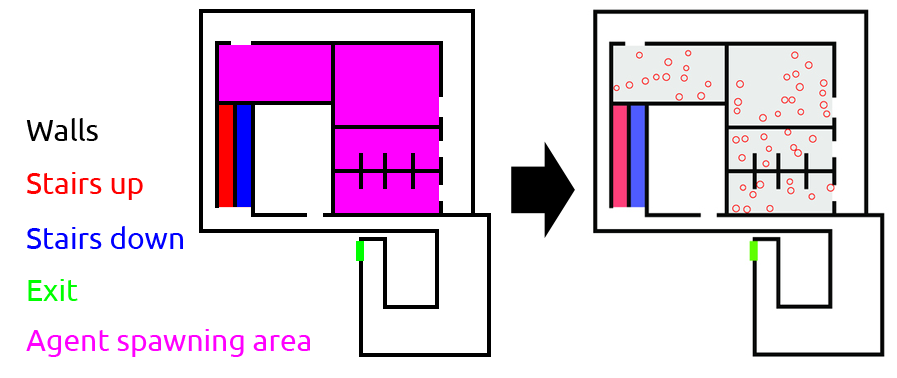
\includegraphics[width=\textwidth]{./images/config_floor_description.png}
\caption{Left the building floor image and right how it looks when the
simulation is running} 
\label{building floor image}
\end{figure}

Since \textit{MATLAB} is not really object-oriented, we used a big data structure (called
data) that includes all internal data that we use (eg. the floors and agents).
It is passed as an argument for every function that needs it.

\subsection{Pathfinding}
As described in \cite{SFMPD}, the agents always try to reach their desired destination
using the shortest possible path. As we use raster graphics to encode simulation data,
we decided to use the same discrete grid to compute the nearest path to an exit for every point approximately.
Mathematically, this can be expressed as an partial differential equation, the 2D Eikonal equation (equation \ref{eq:eikonal}).

\begin{equation} \label{eq:eikonal}
\|\mathbf{\nabla} d(\mathbf{x})\|=1 \quad d:\!\mathbb{R}^{2}\to\mathbb{R},\mathbf{x}\in\mathbb{R}^{2}
\end{equation}

The solution $d(\mathbf{x})$ now gives the distance to the nearest exit point, its
negative gradient $-\mathbf{\nabla}d(\mathbf{x})$ therefor always points in the 
direction of the shortest path towards the desired exit. There are mainly two
competitive agorithms for solving this equation efficiently. First there is the
\textit{Fast Marching} method, a specialized version of Dijkstra's well known 
algorithm \cite{dijkstra59a}. The alternative is \textit{Fast Sweeping}, which 
leads to a much simpler implementation, faster calculation and better algorithmic
complexity of $O(n)$ instead of $O(n\log n)$ with respect to the discretization size.
We therefor implemented an efficient \textit{Fast Sweeping} method, closly following
\cite{Zhao04afast} as a basis of our pathfinding and repulsive wall forces. The 
algorithm uses an upwind finite difference scheme where our mesh is defined by 
the input images. The implementation was done \textit{C} and not directly in
\textit{MATLAB}, using optimized boundary condition handling for our pruposes.
Our benchmarks showed a high speed increase compared to other Eikonal solvers,
e.g. the "Accurate Fast Marching" implementation as found at \textit{MATLAB CENTRAL}
\cite{fastmarching}.


\subsection{Profiling \& Optimization}


Using the \textit{Profiler}-function of \textit{MATLAB}, we were able to discuss
the efficiency of our implementation. The image \vref{cab profile} shows the
time consumption for the calculation of the evacuation of 2 floors (ETH
CAB-Building Floors E and F) within 4087 seconds.

The first version of our simulation showed a different profiling behaviour: The
functions \verb+interp2+ and \verb+addAgentRepulsiveForce+ were at the top and
thus needed most of the calculation time. Now, after our improvements, they are
further down in the profiling ranking, meaning they are more efficient. These
improvements decreased the time for simulation significantly.

\begin{figure}[h]
\centering
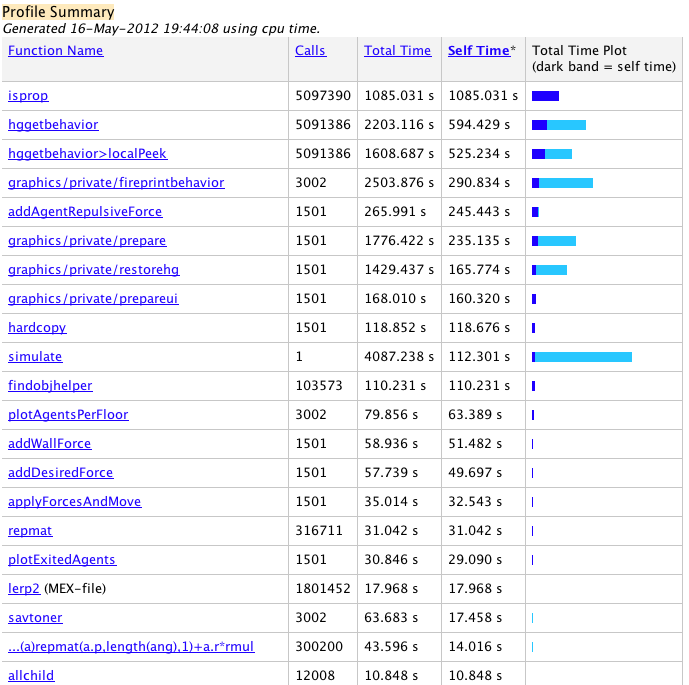
\includegraphics[width=0.8\textwidth]{./images/profiler.png}
\caption{Profile of the calculation for the CAB-Building with 300 agents over 3 different floors} 
\label{cab profile}
\end{figure}

\subsubsection{Parallelization}

We tried to optimize the code using the parallel for-loop parfor in \textit{MATLAB}. In
the function applyForcesAndMove we replaced the for-loop over the agents with
parfor. We measured the time using an input with 200 agents on a 4 core machine
using 5 \textit{MATLAB} workers. The result was that the parfor version was even slightly
slower than the serial version. The reason for this is how \textit{MATLAB} implements
parfor: all the memory that is used by a worker must be sent to this worker.
Each agent must access the building floor image randomly and this creates a
large amount of memory that must be transferred to each worker, which leads to a
decreasing performance.
This is why we decided not to use parfor or any other parallelization in our
implementation.

\subsubsection{Replacing \textit{MATLAB} standard functions}

Through our first messures, we realised that the function \verb+interp2+
consumed a lot of resources and time. We decided to create our own operator
called \verb+lerp2+ (written in \textit{C}) that interpolates between data points. It finds values of a
two-dimensional function interpolating the data at intermediate points bilinearly.
Here the different given data points are the current values of the frame $i-1$
for the frame $i$. 

\subsubsection{Range Tree}
The most time consuming part in our program is the calculation of the interaction
forces between the agents, at least if their count is high enough. To reduce the
natural complexity of order $O(n^{2})$ of this inter-agent interaction, we can clamp forces
with little effect, e.g. in our implementation all forces smaller than $ 10^{4}\newton$.
As their exponentially decreasing, the distance in which the forces need to be adressed
is only several meters, so a big part of them can just be ignored without introducing 
a significant error.

To get all agents influenced by another agent by a force bigger than a threshold, we need to be able
to search neighbours of any agent within a given distance. To efficiently query 
these agents, we implemented a 2D \textit{Range Tree} in \textit{C}, which allows query times
of order $O(\log^{2} n+k)$, where $n$ is the total number of agents and $k$ is the number of
queried agents \cite{algdat}. In larger simulations this reduces simulation times by a significant factor.

\section{Simulation Results and Discussion}

\subsection{Expected Results}

We expect the stairs and the main building exit to be the bottlenecks. The
amount of people in lower levels is increasing with time until a certain point,
when most of the people have exited the building. Also we think that if the 
velocity of the people is higher, jams at the exit will increase.


\subsection{Simulation Results}

% felix
%aehnlichkeit zu helbling paper 
%manche agents bleiben in tuere stecken -> anpassen der parameter noetig
% generell: sieht realistisch aus
%As expected the main exit & stairs becomes a bottleneck...
%TODO: Discussion
% vergleich 2/3 floors cab: bottleneck treppe


% felix
\subsubsection{Comparison to previous projects}
% vergleich mit anderem msssm project (simulation mit gleichem input)


\begin{figure}[h]
\centering
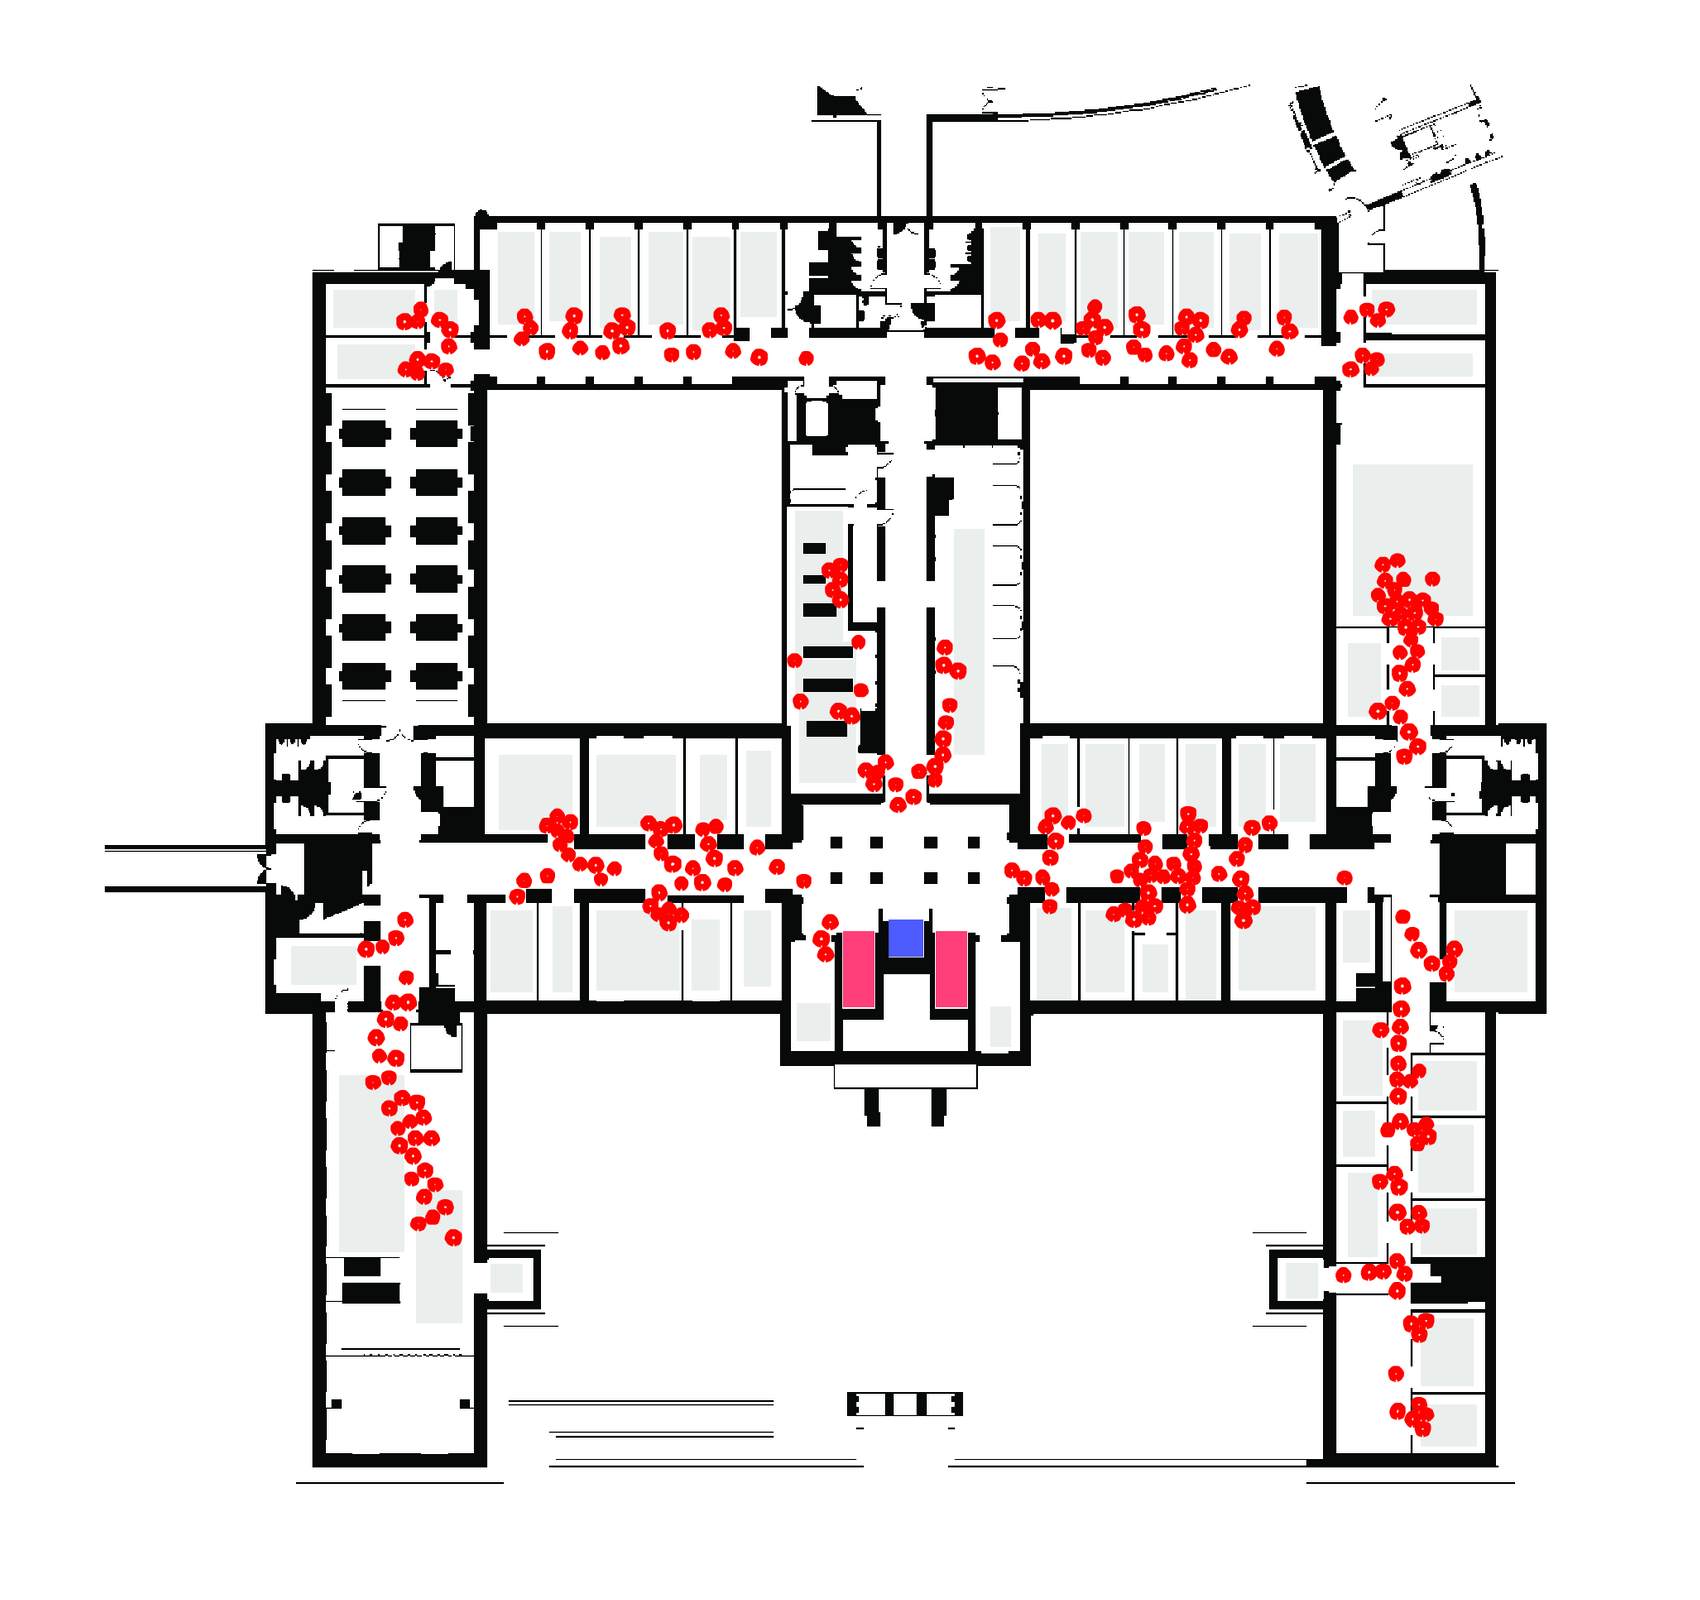
\includegraphics[width=0.8\textwidth]{./images/cab1.png}
\caption{Visualisation of evacuation in the CAB Building E Floor} 
\label{cab1}
\end{figure}


\subsection{Improvements}
%beat
%ausgaenge manchmal zu eng fuer manche agents
% agents nehmen nebenausgang obwohl hauptausgang frei ist
% panic factor nicht implementiert
% zu grosser timestep fuert zu instabilitaet (billiard spiel)
% alle agents sind gleich schnell
% simulation wird mit der zeit immer langsamer (plotten)

Non expected reactions (i.e. paranoia, desesperation or creativity) have not been consider by
making this model and we are sure that in the reality this factors have also a big importance.
This is a point where this work could be improved. Nevertheless, we believe that this project
gives a good prespective in matters of evacuation potential and security.

\section{Summary and Outlook}

In this section we would like to thank the MSSSM-Group from the ETH in Zurich, Switzerland
directed by Karsten Donnay and Stefano Balietti for their engagement in the lecture
"Modeling and Simulating Social Systems with \textit{MATLAB}" during the Spring Semester 2012.
This project helped us to understand that the human behavior is a difficult subject to formalize.


%TODO: Rückblick aufs projekt & Danksagung

\section{References}

\begin{thebibliography} {9}
	
	\bibitem{Zhao04afast} Zhao, Hongkai (2004): A Fast Sweeping Method for Eikonal Equations.
	\bibitem{SFMPD} Helbling, Dirk - Molnar, Peter (1995): Social Force Model for Pedestrians Dynamics.
	\bibitem{AACIBF} Helbling, Dirk, Johnson, Anders (2006): Analytical Approach to Continuous and Intermittent Bottleneck Flows.
	\bibitem{ACPPD} Schadschneider, Andreas et al. (2002): CA Approach to Collective Phenomena in Pedestrian Dynamics.	
	\bibitem{DCD} Helbling, Dirk, Johansson, Anders (2007): Dynamics of crowd disasters: An empirical Study.
	\bibitem{SDFEP} Helbling, Dirk et al. (2000): Simulating dynamical features of escape panic.
	\bibitem{SPCD} Helbling, Dirk et al. (2005): Self-Organized Pedestrian Crowd Dynamics: Experiments, Simulations, and Design Solutions.
	\bibitem{dijkstra59a} Dijkstra, Edsger W. (1959): A Note on Two Problems in Connexion with Graphs.
	\bibitem{fastmarching} Kroon, Dirk-Jan (2011): http://www.mathworks.com/matlabcentral/fileexchange/24531-accurate-fast-marching
	\bibitem{algdat} Ottmann, Thomas, Widmayer, Peter (2002): Algorithmen und Datenstrukturen, 4. Auflage.

\end{thebibliography}

% use \cite{SFMPD} for citation

\section{Appendix}

\subsection{Code}

% define colors
\definecolor{commentcolor}{RGB}{89, 168, 89}
\definecolor{keywordcolor}{RGB}{68, 68, 255}
\definecolor{stringcolor}{RGB}{205, 139, 247}
\definecolor{numbercolor}{RGB}{128, 128, 128}
\definecolor{bgcolor}{RGB}{245, 248, 253}

% define listings style
\lstset{
  language=Matlab,
  basicstyle=\footnotesize\ttfamily,
  numbers=left,
  numberstyle=\tiny\color{numbercolor},
  stepnumber=2,
  numbersep=5pt,
  backgroundcolor=\color{bgcolor},
  showspaces=false, 
  showstringspaces=false,
  showtabs=false,
  frame=lines,
  rulecolor=\color{black},
  tabsize=2,
  captionpos=b,
  breaklines=true,
  breakatwhitespace=true,
  title=\lstname,
  commentstyle=\color{commentcolor},
  keywordstyle=\color{keywordcolor},
  stringstyle=\color{stringcolor}
}

\subsubsection{\textit{MATLAB} code}

% code is ordered alphabetically by file name...

\lstinputlisting[caption=addAgentRepulsiveForce.m]{../code/addAgentRepulsiveForce.m}
\lstinputlisting[caption=addDesiredForce.m]{../code/addDesiredForce.m}
\lstinputlisting[caption=addWallForce.m]{../code/addWallForce.m}
\lstinputlisting[caption=applyForcesAndMove.m]{../code/applyForcesAndMove.m}
\lstinputlisting[caption=checkForIntersection.m]{../code/checkForIntersection.m}
\lstinputlisting[caption=compileC.m]{../code/compileC.m}
\lstinputlisting[caption=initAgents.m]{../code/initAgents.m}
\lstinputlisting[caption=initEscapeRoutes.m]{../code/initEscapeRoutes.m}
\lstinputlisting[caption=initialize.m]{../code/initialize.m}
\lstinputlisting[caption=initWallForces.m]{../code/initWallForces.m}
\lstinputlisting[caption=loadConfig.m]{../code/loadConfig.m}
\lstinputlisting[caption=plotAgentsPerFloor.m]{../code/plotAgentsPerFloor.m}
\lstinputlisting[caption=plotExitedAgents.m]{../code/plotExitedAgents.m}
\lstinputlisting[caption=plotFloor.m]{../code/plotFloor.m}
\lstinputlisting[caption=simulate.m]{../code/simulate.m}

\subsubsection{\textit{C} code}

\lstinputlisting[language=C,caption=createRangeTree.c]{../code/createRangeTree.c}
\lstinputlisting[language=C,caption=fastSweeping.c]{../code/fastSweeping.c}
\lstinputlisting[language=C,caption=getNormalizedGradient.c]{../code/getNormalizedGradient.c}
\lstinputlisting[language=C,caption=lerp2.c]{../code/lerp2.c}
\lstinputlisting[language=C,caption=rangeQuery.c]{../code/rangeQuery.c}
\lstinputlisting[language=C,caption=tree.h]{../code/tree.h}
\lstinputlisting[language=C,caption=tree\_build.h]{../code/tree_build.h}
\lstinputlisting[language=C,caption=tree\_build.c]{../code/tree_build.c}
\lstinputlisting[language=C,caption=tree\_free.c]{../code/tree_free.c}
\lstinputlisting[language=C,caption=tree\_query.h]{../code/tree_query.h}
\lstinputlisting[language=C,caption=tree\_query.c]{../code/tree_query.c}
\lstinputlisting[language=C,caption=tree\_types.h]{../code/tree_types.h}



\end{document}  



 
